\chapter{Weitere FEM-Ergebnisse}\label{sec:mehrFEM}
Die Abbildungen \ref{abb_AnhangFEM1} bis \ref{abb_AnhangFEM2} zeigen die FEM-Ergebnisse beim maximalen Lastfall für die endgültige Gitter und Halterungsstruktur. Es wird sowohl der Tal- als auch der Berg-Typus in allen Positionen und beim maximalen Lastvielfachen gezeigt.\\
Abbildung \ref{abb_AnhangFEM3} zeigt die Belastungen in der Baugruppe der Hubstange beim maximalen Lastfall.
\begin{figure}[h]
	\begin{minipage}[t]{0.5\linewidth}
		\centering
		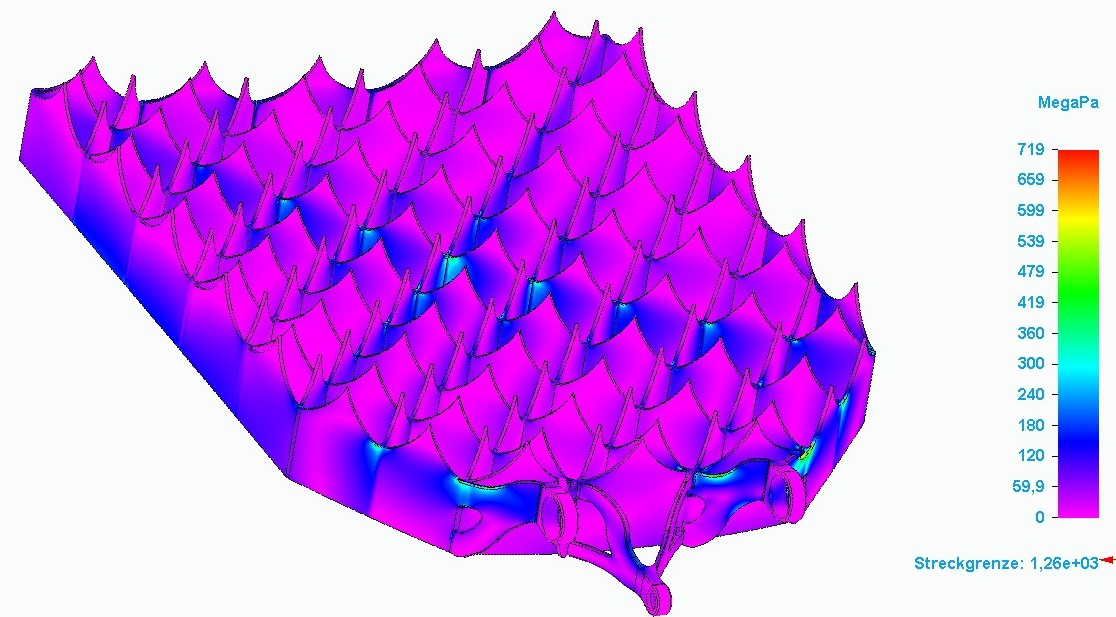
\includegraphics[width=0.95\textwidth]{D1 3.9 t.jpg}
		\caption{Tal-Typus D1 (max: 719 MPa)}
		\label{abb_AnhangFEM1}
	\end{minipage}
	\hfill
	\begin{minipage}[t]{0.5\linewidth}
		\centering
		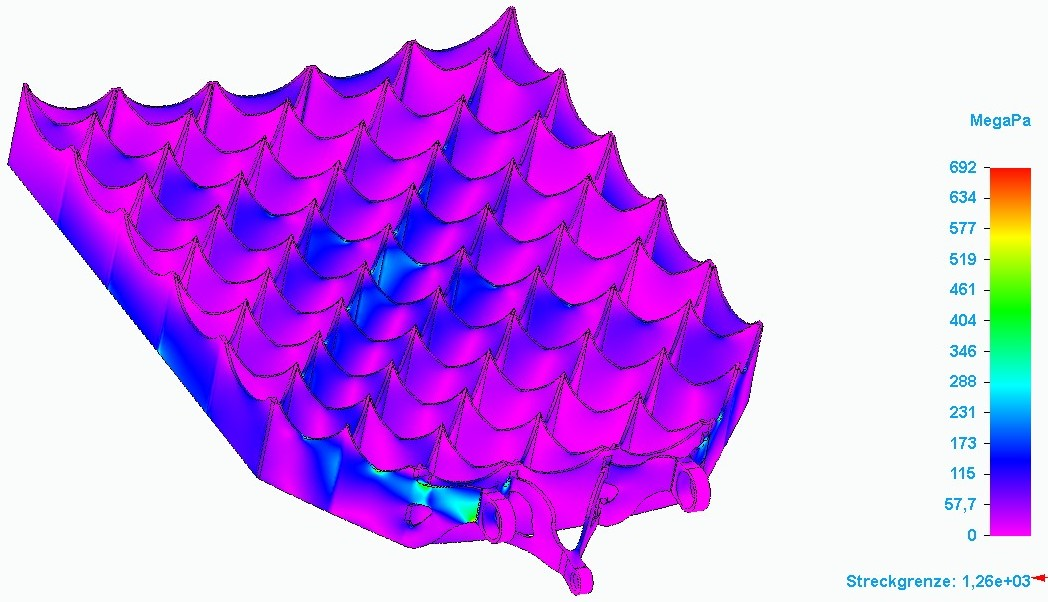
\includegraphics[width=0.95\textwidth]{D1 3.9 b.jpg}
		\caption{Berg-Typus D1 (max: 692 MPa)}
	\end{minipage}
\end{figure}
\begin{figure}[h]
\begin{minipage}[t]{0.5\linewidth}
	\centering
	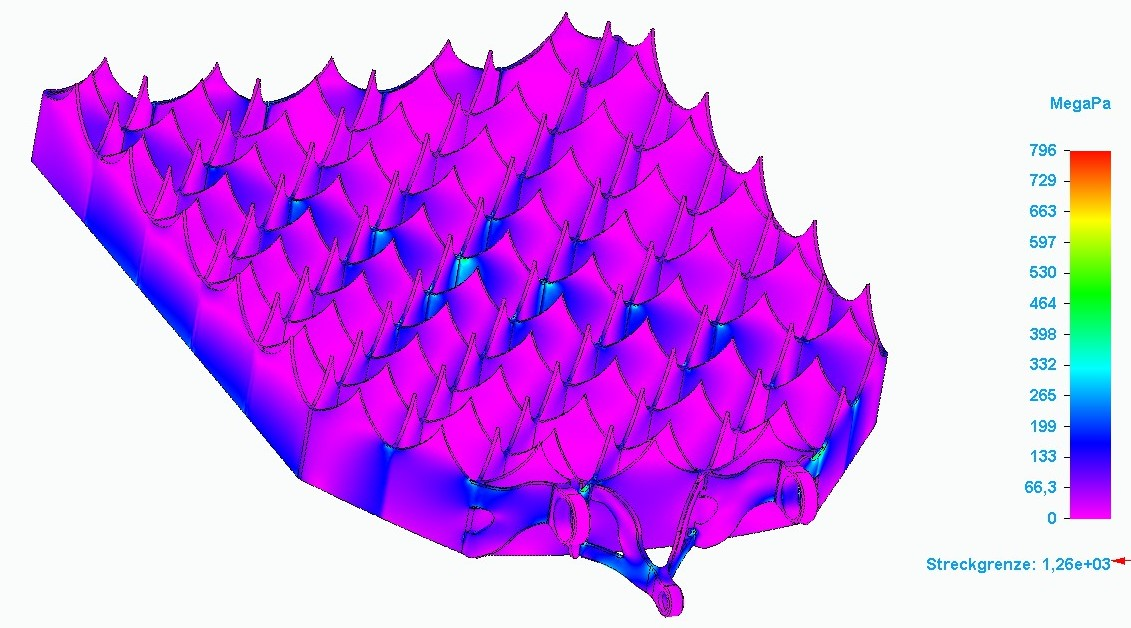
\includegraphics[width=0.95\textwidth]{D2 3.9 t.jpg}
	\caption{Tal-Typus D2 (max: 796 MPa)}
\end{minipage}
\hfill
\begin{minipage}[t]{0.5\linewidth}
	\centering
	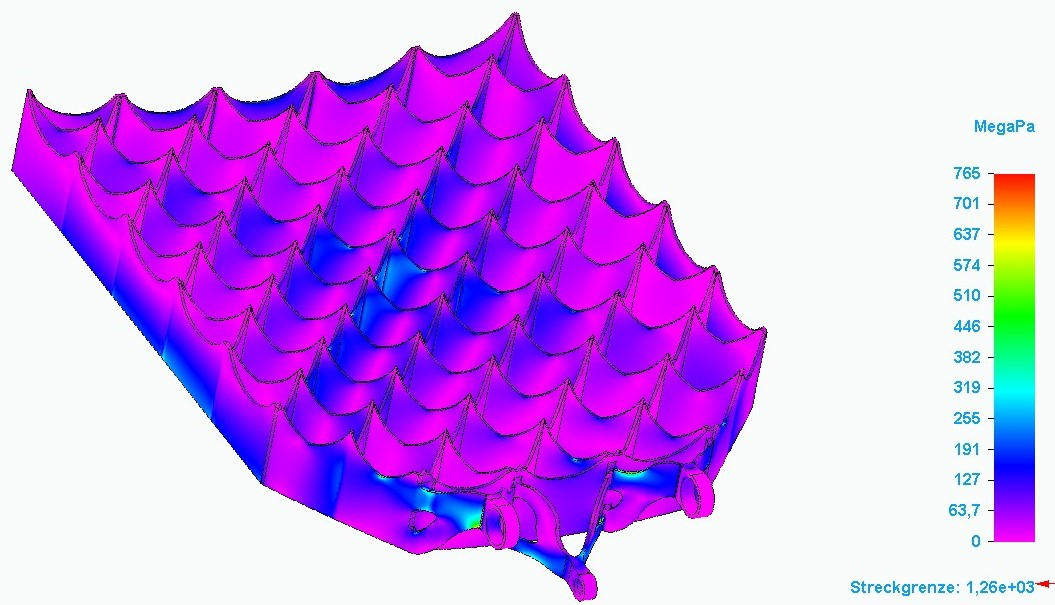
\includegraphics[width=0.95\textwidth]{D2 3.9 b.jpg}
	\caption{Berg-Typus D2 (max: 765 MPa)}
\end{minipage}
\end{figure}
\begin{figure}[h]
\begin{minipage}[t]{0.5\linewidth}
	\centering
	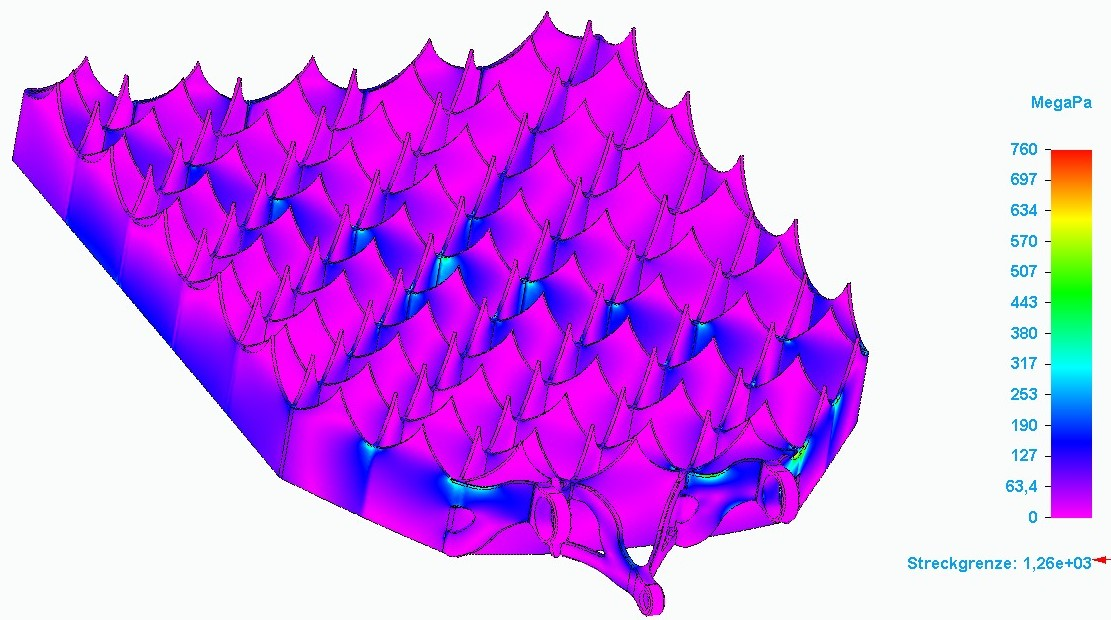
\includegraphics[width=0.95\textwidth]{R1 3.9 t.jpg}
	\caption{Tal-Typus R1 (max: 760 MPa)}
\end{minipage}
\hfill
\begin{minipage}[t]{0.5\linewidth}
	\centering
	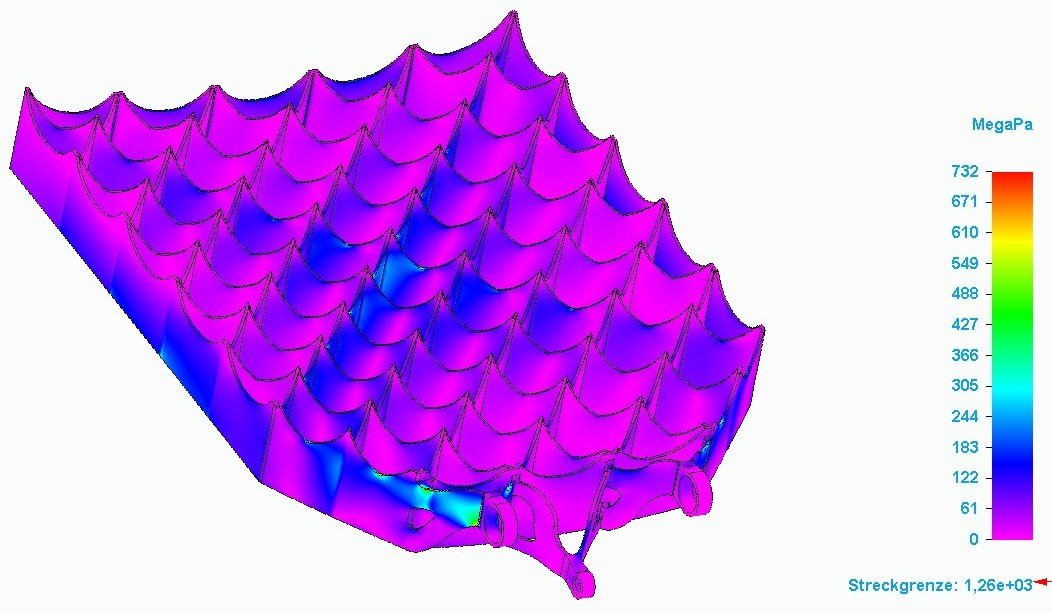
\includegraphics[width=0.95\textwidth]{R1 3.9 b.jpg}
	\caption{Berg-Typus R1 (max: 732 MPa)}
\end{minipage}
\end{figure}
%
%
\begin{figure}[h]
\begin{minipage}[t]{0.5\linewidth}
	\centering
	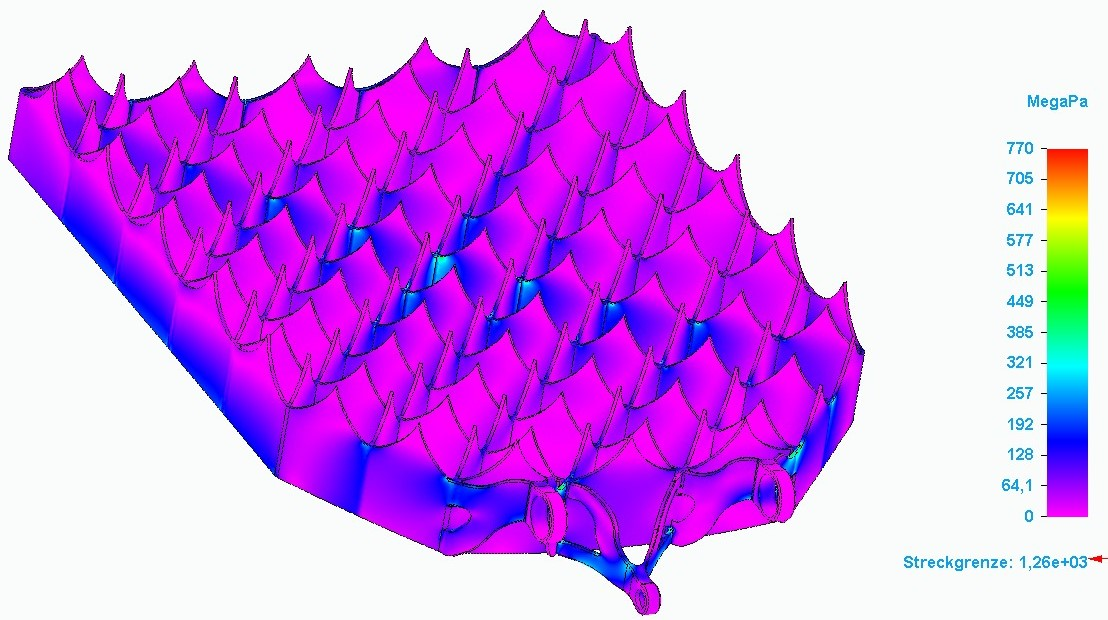
\includegraphics[width=0.95\textwidth]{R2 3.9 t.jpg}
	\caption{Tal-Typus R2 (max: 770 MPa)}
\end{minipage}
\hfill
\begin{minipage}[t]{0.5\linewidth}
	\centering
	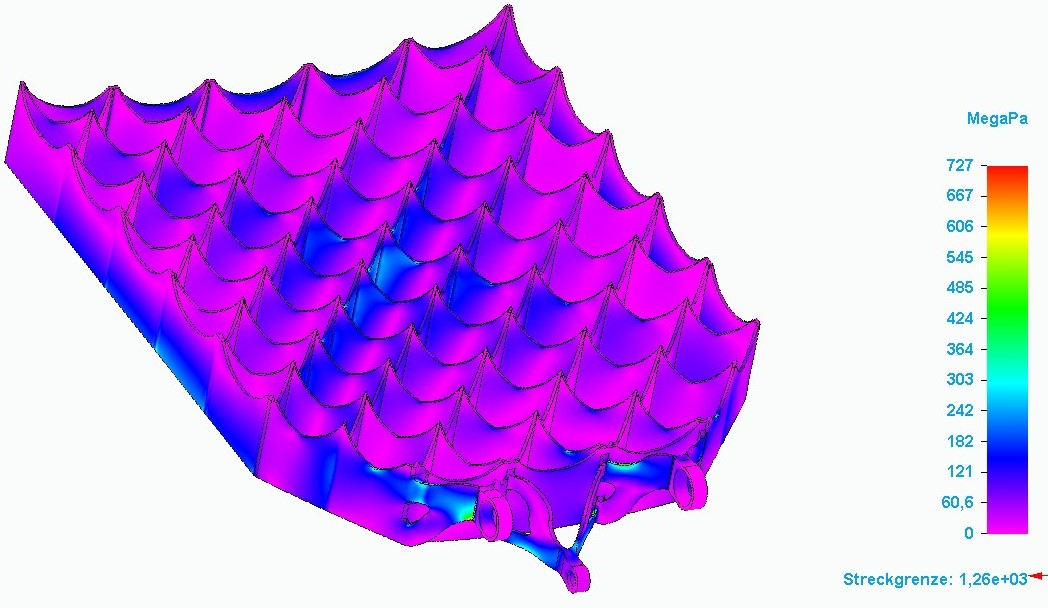
\includegraphics[width=0.95\textwidth]{R2 3.9 b.jpg}
	\caption{Berg-Typus R2 (max: 727 MPa)}
\end{minipage}
\end{figure}
\begin{figure}[h]
\begin{minipage}[t]{0.5\linewidth}
	\centering
	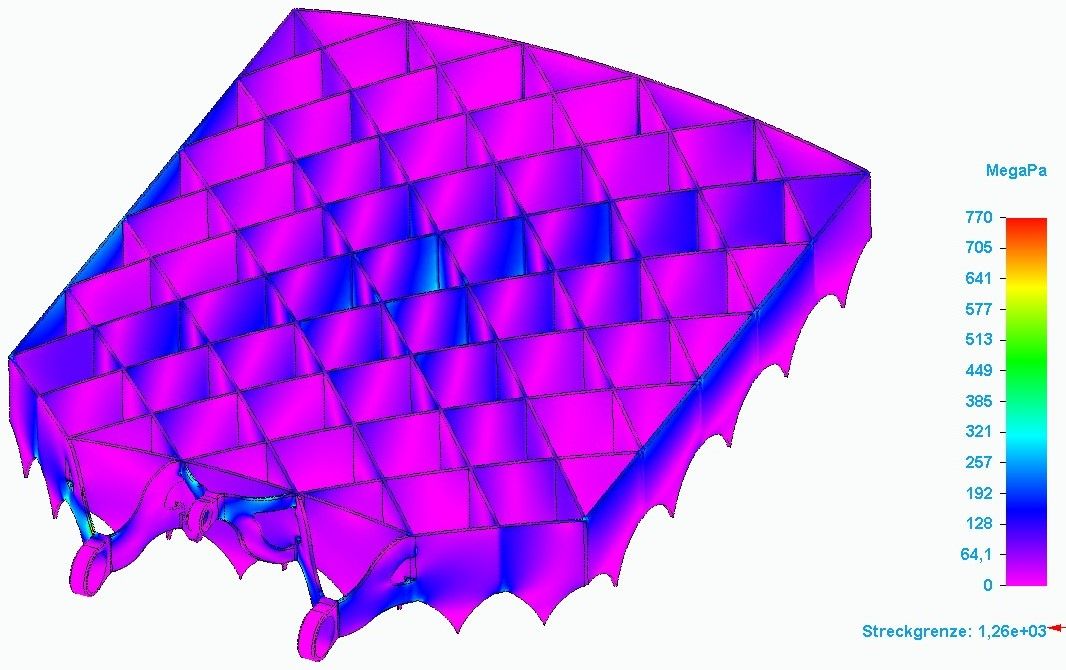
\includegraphics[width=0.95\textwidth]{20g 3.9 t.jpg}
	\caption{Tal-Typus beim maximalen Lastvielfachen (max: 770 MPa)}
\end{minipage}
\hfill
\begin{minipage}[t]{0.5\linewidth}
	\centering
	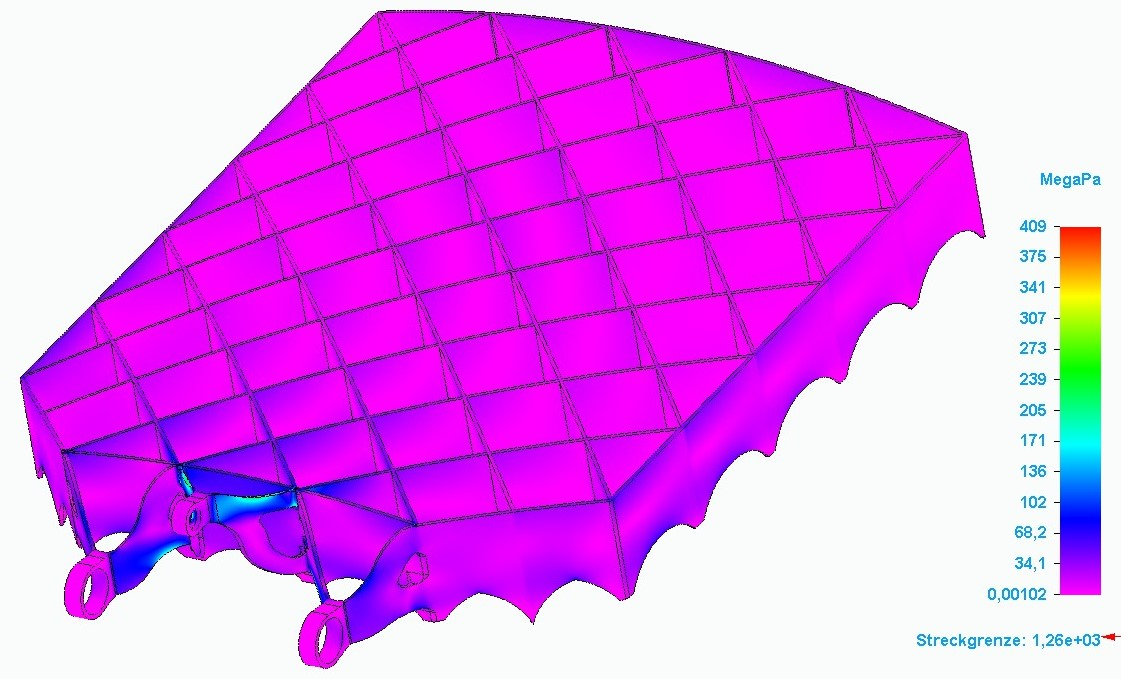
\includegraphics[width=0.95\textwidth]{20g 3.9 b.jpg}
	\caption{Berg-Typus beim maximalen Lastvielfachen (max: 409 MPa)}
	\label{abb_AnhangFEM2}
\end{minipage}
\end{figure}
\begin{figure}[h]
\centering
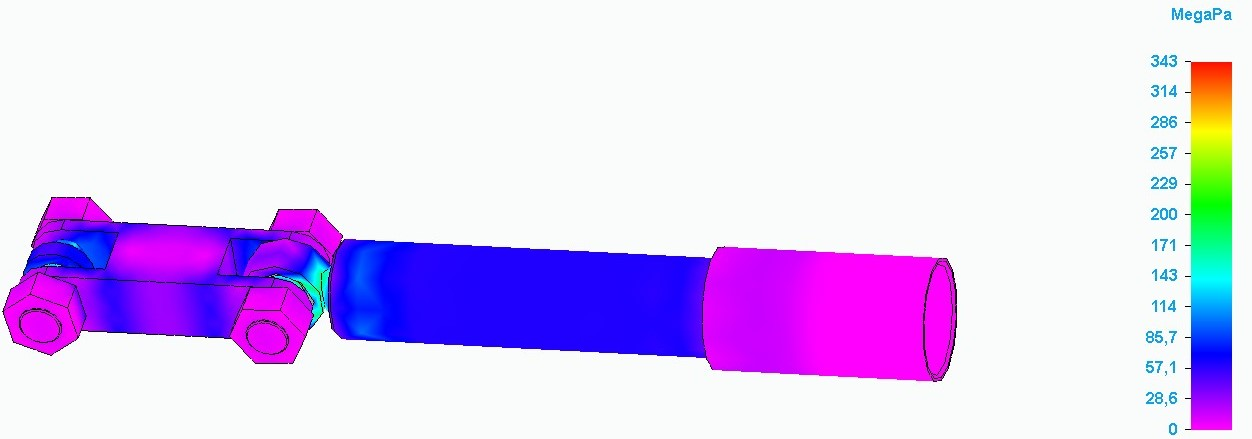
\includegraphics[width=0.8\textwidth]{FEM Hub.jpg}
\caption{Ergebnisse der FEM Berechnung der Hub-Baugruppe beim maximalen Lastvielfachen (max: 343 MPa)}
\label{abb_AnhangFEM3}
\end{figure}